% !TEX root = Thesis.tex

\chapter{Preliminaries}\label{chap:prelim}

  \newtheorem{defi}{Definition}

  In this section, we first raise the motivation to utilize triangulation for analog layout migration in Chapter~\ref{sec:WhyCDT}, and later review the planar straight-line graph (PSLG) and the corresponding constrained Delaunay triangulation (CDT)~\cite{CDT} in Chapter~\ref{sec:Review}. In the end, we define the analog layout prototyping problem in Chapter~\ref{sec:problem}.

  \section{Routing Preservation with Planar Triangulation}\label{sec:WhyCDT}

    To facilitate the routing preservation in the existing layout, the relationship between routing wires and placement blocks is crucial. The triangulation of layout plane is used to take down the correlation. Fig.~\ref{fig:WhyCDT} depicts that the updated triangular edges can retain the routing behavior among blocks after shrinking and stretching. Therefore, planar triangulation is applied to our analog layout migration mechanism.

    \begin{figure}[ht]
      \begin{center}
        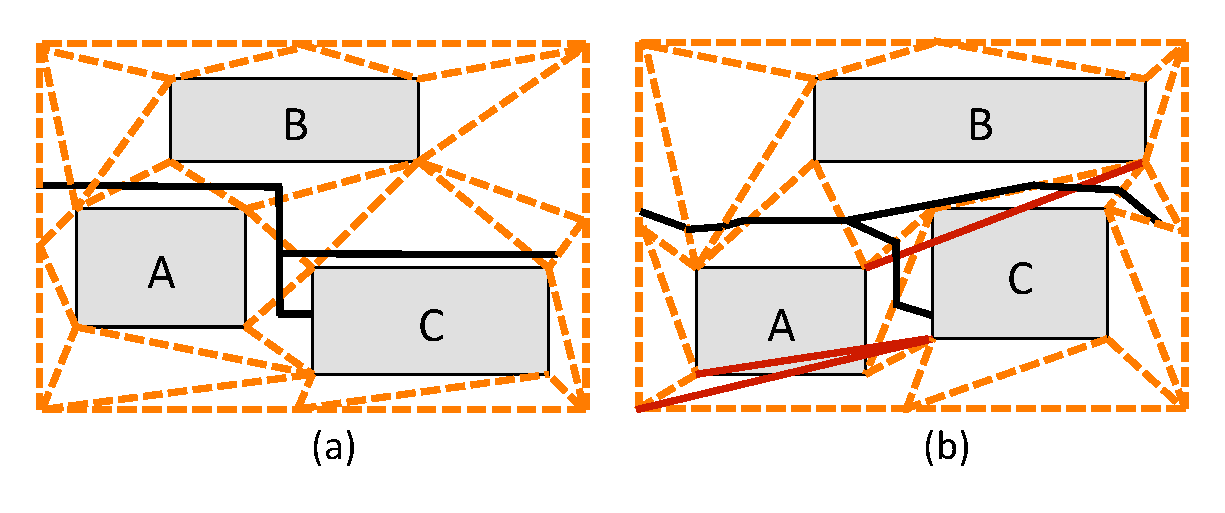
\includegraphics[width=\textwidth]{Fig/WhyCDT.eps}
        \caption{Illustration of triangulation to take down the correlation between placement and routing. (a). The existing layout with triangles at routing channel. (b) The migrated layout with updated triangular edges and recovering routing paths.}
        \label{fig:WhyCDT}
      \end{center}
    \end{figure}

  \section{Review of PSLG and CDT}\label{sec:Review}

    In order to describe the analog layout design as a planar straight-line graph (PSLG), we briefly define PSLG as follows:

    \begin{defi}\label{defi:PSLG}
      A PSLG is a graph $G(V,E)$, which can be embedded in the plane without any crossing. Every edge $E$ in $G$ is a straight segment, where $V$ implies all the vertices in $G$ and $E$ implies all the edges connected to $V$. 
    \end{defi}

    By definition~\ref{defi:PSLG}, we can use PSLG to describe the placement of the analog layout with several rectangles and polygons. Furthermore, polygons decomposition is facilitated by decomposing into simpler components such as triangles. The triangulation can be generalized to a PSLG, where the entire plane is decomposed into triangles. The triangulation is defined in the following definition.

    \begin{defi}\label{defi:Triangulation}
      Triangulation is a process to produce an updated PSLG $G'(V'E')$ out of a given PSLG $G(V,E)$, such that each edge $e' \in E'$ is exactly a triangular edge.
    \end{defi}

    The complexity of triangulation is $O(n\log n)$, which is well explained in \cite{CDT}. We further look for a quality triangulation instead of triangles with arbitrary shapes. Therefore, the Delaunay Triangulation generates a set of points satisfying the empty circumcircle property, which maximizes the minimum angles. Therefore, CDT can minimize the number of triangles with small angles among placement blocks in the layout. In other words, CDT reduces the total number of triangular angles the routing wires should intersect. Additionally, in a practical analog layout problem, not all polygons and rectangles are supposed to be decomposed into triangles, such as obstacles and devices. The generalized Delaunay triangulation, which is also called constrained Delaunay triangulation (CDT), fit better for our requirement. 

    According to above definitions, it is possible to decompose the analog layout with obstacles and routing channels into convex holes and triangles, where the quality triangles are capable of preserving the across wires. 

  \section{Problem Description}\label{sec:problem}

    In this work, we aim at an analog layout migration problem by layout prototyping. 
    The problem can be described as follows:

    \newcommand{\tabincell}[2]{\begin{tabular}{@{}#1@{}}#2\end{tabular}}
    \newsavebox{\tablebox}


    \begin{itemize}
    \item 
    {\bf Analog Layout Migration Problem} 
    Given a source layout $L$ with technology information $T$, the main purpose is to produce a new $L'$ on target technology $T'$. The original layout $L$ comprises a set of placement modules $M$ and nets $N$, which consisting of at least one wire segment. Our objective is to provide multiple layout solutions. These layout solutions make more opportunities for designers to generate the appropriate layout much faster.
    \end{itemize}

    